\documentclass{article}
% packages
\usepackage[utf8]{inputenc}
\usepackage{amsmath,amssymb}
\usepackage{graphicx} 
\usepackage{subcaption}
\usepackage{xspace}
\usepackage{color}
\usepackage{soul}
\usepackage{geometry}
\usepackage{float}
\usepackage{booktabs}
\usepackage{multirow}
\usepackage{algorithm}
\usepackage[noend]{algpseudocode}
\usepackage{listings}
\usepackage{natbib}
\usepackage[colorlinks,citecolor=blue,bookmarks=false]{hyperref}
\geometry{a4paper,total={170mm,257mm},left=20mm,top=20mm}

% shortcuts for bold characters (vectors, matrices)
\newcommand{\ba}{\mathbf{a}}\newcommand{\bA}{\mathbf{A}}
\newcommand{\bb}{\mathbf{b}}\newcommand{\bB}{\mathbf{B}}
\newcommand{\bc}{\mathbf{c}}\newcommand{\bC}{\mathbf{C}}
\newcommand{\bd}{\mathbf{d}}\newcommand{\bD}{\mathbf{D}}
\newcommand{\be}{\mathbf{e}}\newcommand{\bE}{\mathbf{E}}
\newcommand{\bff}{\mathbf{f}}\newcommand{\bF}{\mathbf{F}} %\bf already taken
\newcommand{\bg}{\mathbf{g}}\newcommand{\bG}{\mathbf{G}}
\newcommand{\bh}{\mathbf{h}}\newcommand{\bH}{\mathbf{H}}
\newcommand{\bi}{\mathbf{i}}\newcommand{\bI}{\mathbf{I}}
\newcommand{\bj}{\mathbf{j}}\newcommand{\bJ}{\mathbf{J}}
\newcommand{\bk}{\mathbf{k}}\newcommand{\bK}{\mathbf{K}}
\newcommand{\bl}{\mathbf{l}}\newcommand{\bL}{\mathbf{L}}
\newcommand{\bm}{\mathbf{m}}\newcommand{\bM}{\mathbf{M}}
\newcommand{\bn}{\mathbf{n}}\newcommand{\bN}{\mathbf{N}}
\newcommand{\bo}{\mathbf{o}}\newcommand{\bO}{\mathbf{O}}
\newcommand{\bp}{\mathbf{p}}\newcommand{\bP}{\mathbf{P}}
\newcommand{\bq}{\mathbf{q}}\newcommand{\bQ}{\mathbf{Q}}
\newcommand{\br}{\mathbf{r}}\newcommand{\bR}{\mathbf{R}}
\newcommand{\bs}{\mathbf{s}}\newcommand{\bS}{\mathbf{S}}
\newcommand{\bt}{\mathbf{t}}\newcommand{\bT}{\mathbf{T}}
\newcommand{\bu}{\mathbf{u}}\newcommand{\bU}{\mathbf{U}}
\newcommand{\bv}{\mathbf{v}}\newcommand{\bV}{\mathbf{V}}
\newcommand{\bw}{\mathbf{w}}\newcommand{\bW}{\mathbf{W}}
\newcommand{\bx}{\mathbf{x}}\newcommand{\bX}{\mathbf{X}}
\newcommand{\by}{\mathbf{y}}\newcommand{\bY}{\mathbf{Y}}
\newcommand{\bz}{\mathbf{z}}\newcommand{\bZ}{\mathbf{Z}}

% shortcuts for bold greek characters (vectors, matrices)
\newcommand{\balpha}{\boldsymbol{\alpha}}\newcommand{\bAlpha}{\boldsymbol{\Alpha}}
\newcommand{\bbeta}{\boldsymbol{\beta}}\newcommand{\bBeta}{\boldsymbol{\Beta}}
\newcommand{\bgamma}{\boldsymbol{\gamma}}\newcommand{\bGamma}{\boldsymbol{\Gamma}}
\newcommand{\bdelta}{\boldsymbol{\delta}}\newcommand{\bDelta}{\boldsymbol{\Delta}}
\newcommand{\bepsilon}{\boldsymbol{\epsilon}}\newcommand{\bEpsilon}{\boldsymbol{\Epsilon}}
\newcommand{\bzeta}{\boldsymbol{\zeta}}\newcommand{\bZeta}{\boldsymbol{\Zeta}}
\newcommand{\beeta}{\boldsymbol{\eta}}\newcommand{\bEta}{\boldsymbol{\Eta}} % \beta already taken
\newcommand{\btheta}{\boldsymbol{\theta}}\newcommand{\bTheta}{\boldsymbol{\Theta}}
\newcommand{\biota}{\boldsymbol{\iota}}\newcommand{\bIota}{\boldsymbol{\Iota}}
\newcommand{\bkappa}{\boldsymbol{\kappa}}\newcommand{\bKappa}{\boldsymbol{\Kappa}}
\newcommand{\blambda}{\boldsymbol{\lambda}}\newcommand{\bLambda}{\boldsymbol{\Lambda}}
\newcommand{\bmu}{\boldsymbol{\mu}}\newcommand{\bMu}{\boldsymbol{\Mu}}
\newcommand{\bnu}{\boldsymbol{\nu}}\newcommand{\bNu}{\boldsymbol{\Nu}}
\newcommand{\bxi}{\boldsymbol{\xi}}\newcommand{\bXi}{\boldsymbol{\Xi}}
\newcommand{\bomikron}{\boldsymbol{\omikron}}\newcommand{\bOmikron}{\boldsymbol{\Omikron}}
\newcommand{\bpi}{\boldsymbol{\pi}}\newcommand{\bPi}{\boldsymbol{\Pi}}
\newcommand{\brho}{\boldsymbol{\rho}}\newcommand{\bRho}{\boldsymbol{\Rho}}
\newcommand{\bsigma}{\boldsymbol{\sigma}}\newcommand{\bSigma}{\boldsymbol{\Sigma}}
\newcommand{\btau}{\boldsymbol{\tau}}\newcommand{\bTau}{\boldsymbol{\Tau}}
\newcommand{\bypsilon}{\boldsymbol{\ypsilon}}\newcommand{\bYpsilon}{\boldsymbol{\Ypsilon}}
\newcommand{\bphi}{\boldsymbol{\phi}}\newcommand{\bPhi}{\boldsymbol{\Phi}}
\newcommand{\bchi}{\boldsymbol{\chi}}\newcommand{\bChi}{\boldsymbol{\Chi}}
\newcommand{\bpsi}{\boldsymbol{\psi}}\newcommand{\bPsi}{\boldsymbol{\Psi}}
\newcommand{\bomega}{\boldsymbol{\omega}}\newcommand{\bOmega}{\boldsymbol{\Omega}}

% shortcuts for blackboard bold characters (eg, number sets)
\newcommand{\nA}{\mathbb{A}}
\newcommand{\nB}{\mathbb{B}}
\newcommand{\nC}{\mathbb{C}}
\newcommand{\nD}{\mathbb{D}}
\newcommand{\nE}{\mathbb{E}}
\newcommand{\nF}{\mathbb{F}}
\newcommand{\nG}{\mathbb{G}}
\newcommand{\nH}{\mathbb{H}}
\newcommand{\nI}{\mathbb{I}}
\newcommand{\nJ}{\mathbb{J}}
\newcommand{\nK}{\mathbb{K}}
\newcommand{\nL}{\mathbb{L}}
\newcommand{\nM}{\mathbb{M}}
\newcommand{\nN}{\mathbb{N}}
\newcommand{\nO}{\mathbb{O}}
\newcommand{\nP}{\mathbb{P}}
\newcommand{\nQ}{\mathbb{Q}}
\newcommand{\nR}{\mathbb{R}}
\newcommand{\nS}{\mathbb{S}}
\newcommand{\nT}{\mathbb{T}}
\newcommand{\nU}{\mathbb{U}}
\newcommand{\nV}{\mathbb{V}}
\newcommand{\nW}{\mathbb{W}}
\newcommand{\nX}{\mathbb{X}}
\newcommand{\nY}{\mathbb{Y}}
\newcommand{\nZ}{\mathbb{Z}}

% shortcuts for calligraphic characters (sets, index sets, ...)
\newcommand{\cA}{\mathcal{A}}
\newcommand{\cB}{\mathcal{B}}
\newcommand{\cC}{\mathcal{C}}
\newcommand{\cD}{\mathcal{D}}
\newcommand{\cE}{\mathcal{E}}
\newcommand{\cF}{\mathcal{F}}
\newcommand{\cG}{\mathcal{G}}
\newcommand{\cH}{\mathcal{H}}
\newcommand{\cI}{\mathcal{I}}
\newcommand{\cJ}{\mathcal{J}}
\newcommand{\cK}{\mathcal{K}}
\newcommand{\cL}{\mathcal{L}}
\newcommand{\cM}{\mathcal{M}}
\newcommand{\cN}{\mathcal{N}}
\newcommand{\cO}{\mathcal{O}}
\newcommand{\cP}{\mathcal{P}}
\newcommand{\cQ}{\mathcal{Q}}
\newcommand{\cR}{\mathcal{R}}
\newcommand{\cS}{\mathcal{S}}
\newcommand{\cT}{\mathcal{T}}
\newcommand{\cU}{\mathcal{U}}
\newcommand{\cV}{\mathcal{V}}
\newcommand{\cW}{\mathcal{W}}
\newcommand{\cX}{\mathcal{X}}
\newcommand{\cY}{\mathcal{Y}}
\newcommand{\cZ}{\mathcal{Z}}

% references to figures, sections, algorithms, equations, tables
\newcommand{\figref}[1]{Fig.~\ref{#1}}
\newcommand{\secref}[1]{Section~\ref{#1}}
\newcommand{\eqnref}[1]{Eq.~\eqref{#1}}
\newcommand{\tabref}[1]{Table~\ref{#1}}

% standard math operators
\DeclareMathOperator*{\argmax}{argmax~}
\DeclareMathOperator*{\argmin}{argmin~}
\DeclareMathOperator*{\softmax}{softmax}
\DeclareMathOperator*{\sgn}{sgn}
\DeclareMathOperator*{\Tr}{Tr}
\DeclareMathOperator*{\Bias}{Bias}
\DeclareMathOperator*{\Var}{Var}
\DeclareMathOperator*{\diag}{diag}
\DeclareMathOperator*{\Perplexity}{Perplexity}

% mathcal / mathbf shortcuts
\def\mc{\mathcal}
\def\mb{\mathbf}

% total derivative
\def\diff{\mathrm{d}}

% statistical independence symbol (_||_)
\newcommand{\Perp}{\perp\!\!\! \perp}

% shortcuts for: \eg, \ie, \cf, \etc, \vs, \wrt, \dof, \etal, \iid
\makeatletter
\DeclareRobustCommand\onedot{\futurelet\@let@token\@onedot}
\def\@onedot{\ifx\@let@token.\else.\null\fi\xspace}
\def\eg{e.g\onedot} \def\Eg{E.g\onedot}
\def\ie{i.e\onedot} \def\Ie{I.e\onedot}
\def\cf{cf\onedot} \def\Cf{Cf\onedot}
\def\etc{etc\onedot}
\def\vs{vs\onedot}
\def\wrt{wrt\onedot}
\def\dof{d.o.f\onedot}
\def\etal{et~al\onedot}
\def\iid{i.i.d\onedot}
\def\eos{\texttt{\textless EOS\textgreater}}
\makeatother

% nice url font and color
\renewcommand\UrlFont{\color{blue}\rmfamily}

% custom color definitions
\definecolor{darkred}{rgb}{0.8,0,0}
\definecolor{darkgreen}{rgb}{0,0.5,0}
\definecolor{darkblue}{rgb}{0,0,0.7}
\definecolor{darkpurple}{rgb}{0.4,0,0.6}
\definecolor{lightgray}{rgb}{0.92,0.92,0.92}
\definecolor{lightpink}{rgb}{1.00,0.90,0.90}

% command for comments / red highlighting
\newcommand{\red}[1]{\noindent{\color{red}{#1}}}
\newcommand{\white}[1]{\noindent{\color{white}{#1}}}
\newcommand{\green}[1]{\noindent{\color{darkgreen}{#1}}}
\newcommand{\blue}[1]{\noindent{\color{darkblue}{#1}}}

\title{Ko\c{c} University \\COMP547 Deep Unsupervised Learning\\ Lecture Notes\footnote{Instructions borrowed from Andreas Geiger from his notes for his Deep Learning class.}}
\author{Aykut Erdem}
\date{February 28, 2021}

\begin{document}

\maketitle

% set this counter to x-1 where x is the number of the lecture you are writing notes for
\setcounter{section}{0}

\section{Instructions}

This is the official template for the lecture notes of the COMP547 Deep Unsupervised Learning class in Spring 2021 at Ko\c{c} University. We will continuously consolidate and compile all lecture notes into a single manuscript. The goal is to obtain a manuscript that is comprehensive and mathematically precise to complement the lecture slides and guide the reader/students in better understanding the course materials. These lecture notes should act as a complement to the lecture slides and therefore do not need to necessarily comprise all figures from the lecture slides. They should, however, provide a concise mathematical description of all concepts that have been discussed in the lectures and include the most important illustrations for understanding those. As a rough guideline, the notes for each lecture should be between 8 and 15 pages. Note that every student must submit his/her lecture notes individually, \ie, this task cannot be done in groups. The assignment of students to lecture is done in the beginning of the class, you will be notified which lecture has been assigned to you via email. Note that you must submit the notes for your lecture via Blackboard within 10 days of the official date where the lecture was held.

To start notes for your assigned lecture, please carefully read these instructions. Then make a copy (Menu $\rightarrow$ Copy Project) of this template, erase the instructions and start editing -- directly in Overleaf or using another \LaTeX~editor of your choice. If you haven't used Overleaf or \LaTeX~before, we highly recommend you to use Overleaf instead of a stand-alone Latex editor, and to read \url{https://www.overleaf.com/learn} to get started. \LaTeX~is easy to learn, in particular when using the online editor Overleaf, and it is a useful typesetting tool which will become your friend for writing project reports, Bachelor's or Master's theses. After you are done with writing your lecture notes, download them as a zip file (Menu $\rightarrow$ Source), and submit them via Blackboard.

When you have read this far, I am assuming that you are familiar with the basics of \LaTeX~and the usage of the Overleaf editor. In particular, you know the basic \LaTeX~commands and know the relevant Overleaf shortcuts that help you editing your notes, \eg, the small arrows in the middle are useful for jumping between corresponding locations in the source and pdf file, \etc. For writing your lecture notes, please orient yourself at the structure of the lecture and the lecture slides. Use the exact same notation wherever possible. All formulas on the lecture slides must appear in the lecture notes and must be explained. Make sure to describe the meaning of each mathematical symbol as well as the relevant domains, \eg, $\bx \in \nR^2$ is a vector in 2D space. You may add additional details and derivations if you find this useful for understanding the concepts discussed in the lecture. You can use Mathpix Snip tool (\url{https://mathpix.com}) to grab equations from the lecture slides if needed. In the following, we provide some instructions/best practices for writing your lecture notes. Please also have a look at the current status of the combined lecture notes document to get an idea and ensure consistency with previous sections.

\subsection{Subsections}
\label{sec:subsections}

Each lecture will become a section in this document. To further structure the notes for your lecture, use \texttt{subsections}, where each subsection is numbered exactly the same way as it is in the lecture slides: the section title of lecture 1 should read ``1 Introduction'' and the subsection title of unit 1.2 of lecture 1 should read ``1.2 History of Deep Learning'', \etc. Use the command \texttt{setcounter} in the beginning of this document to adjust the lecture number. Add a label with the name (in the format: \texttt{sec:sectionname}) of each section directly after the section such that you are able to refer to it when needed, \eg, \secref{sec:subsections} or \secref{sec:subsubsections}.

\subsubsection{Subsubsections}
\label{sec:subsubsections}

Use \texttt{subsubsections} to provide a finer granularity to your lecture notes where necessary.

\subsection{Illustrations}

Add illustrations that you like to include into your lecture notes as compressed jpg or png to the folder \texttt{figures/your\_lecture}. Use figure environments with captions and labels. It is a good idea to provide a short description in bold followed by a longer multi-sentence description in regular text as caption as illustrated below. Reference your figures via the \texttt{figref} command (\eg, \figref{fig:universe}) from the main text.

\begin{figure}[h]
\centering
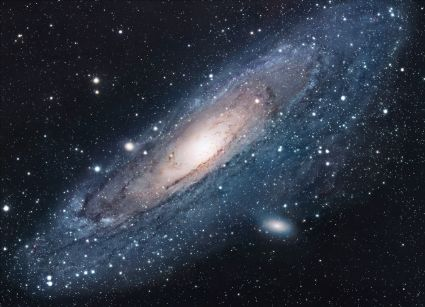
\includegraphics[width=0.8\linewidth]{figures/universe}
\caption{\textbf{The Universe.} An illustration of the universe. It is beautiful.}
\label{fig:universe}
\end{figure}

\subsection{Citations}

Add any paper/journal references which you like to use to \texttt{bibliography.bib}. You can use \url{https://dblp.org/} to find the bibliographic information for papers. Only include the most relevant information (title, authors, year, conference, for journals: journal, volume, number pages) in the bibtex entry. Use shortcut strings for conferences and journals as defined in \texttt{bibliography\_strings.bib}. Inspect the references in \texttt{bibliography.bib} for examples. You can then cite your references using the \texttt{cite} command \cite{Rumelhart1986NATURE}.

\subsection{Equations}

Use a mix of inline math $a=1$ and display math equations
%
\begin{equation}
    b = 2
    \label{eq:b_equals_2}
\end{equation}
%
as you find appropriate. It is a good idea to use inline math equations for short equations that are less important, to specify the domain of a variable or to refer to functions or parameters in the main text. Display math equations (separate line with line number) should be used for important definitions, derivations or longer mathematical expressions. Use numbered equations for display math equations as above. Add labels for referencing them using the \texttt{eqnref} command, \eg, \eqnref{eq:b_equals_2}. Use the \texttt{align} command for multi-line equations. Inspect the sources of the lecture slides (provided in ILIAS) for examples.

\subsection{Preamble / Shortcuts}

Before starting to write, carefully inspect the file \texttt{preamble.tex}. You will find many shortcuts to important commands which will help you in writing legible \LaTeX~source code. Do not invent new commands (\eg, commands for entire mathematical expressions) unless absolutely necessary, but rather use those provided in \texttt{preamble.tex}. Here are some examples:

\begin{itemize}
    \item Vectors and matrices are often expressed using bold face notation: $\bA \bx = \by$
    \item Domains or expectations are often expressed using blackboard characters: $\nR^2, \nZ, \nC, \nE_{x\sim P}[f(x)]$
    \item Sets are sometimes expressed using calligraphic characters: $\cS,\cM$
    \item Probability distributions are often expressed using calligraphic characters: $x \sim \cN(\mu,\sigma)$
    \item The preamble defines shortcuts for argmin/argmax commands, traces and variance operators, \eg:
    \begin{equation}
        x_{min}=\argmin_x x^2 \qquad x_{max}=\argmax_x x^2 \qquad x = \Tr(\bX)
    \end{equation}
    \item Furthermore, there are some shortcuts defined for the most important abbreviations: \eg, \ie, \cf, \etc, \vs, \wrt, \dof, \etal, \iid. Make sure to use those commands.
    \item Add new commands to the preamble only if really necessary and add a comment on why you have introduced them. This will help the TAs consolidating the files. But please try to stick with the overall format and structure of the template as much as possible.
\end{itemize}

\subsection{Additional Packages}

Add additional packages only if really needed. Make sure that these packages are compatible with earlier chapters of the lecture notes (\eg, do not include additional or conflicting algorithm environments).

% bibliography
\bibliographystyle{plain}
\bibliography{bibliography_strings,bibliography_custom}

\end{document}
